\documentclass[thesis.tex]{subfiles}

\chapter{Thực nghiệm và đánh  giá}

\section{Cơ sở dữ liệu}
Để xây dựng cơ sở dữ liệu cho phần thực nghiệm, tác giả tổng hợp và sàng lọc dữ liệu từ ba bộ dữ liệu công khai: ZaloAI, VIVOS Corpus và VLSP ASR 2020.

Bắt đầu từ năm 2018, ZaloAI challenge \cite{ZaloAIChallenge} là một cuộc thi thường niên tập trung vào trí tuệ nhân tạo do Zalo Group, VNG tổ chức. Năm 2020, ZaloAI challenge thử thách các nhà phát triển và kỹ sư học máy Việt Nam với ba bài toán: tóm tắt tin tức, phát hiện biển báo giao thông, và xác thực người nói. Bộ dữ liệu huấn luyện công khai của bài toán xác thực giọng nói bao gồm 400 danh tính tiếng Việt thu thập từ chương trình truyền hình Bạn muốn hẹn hò. Mỗi danh tính có trung bình \textit{26.4} câu nói với phân phối mô tả trong Hình \ref{fig:zaloai}. Bộ dữ liệu tuy đa dạng về mặt độ tuổi giới tính tuy nhiên vẫn còn vấn đề như: trùng lặp danh tính, nhiễu âm thanh như nhạc nền, người nói phía sau, câu nói của danh tính này lẫn vào danh tính kia, ...

\begin{figure}[h]
  \centering
  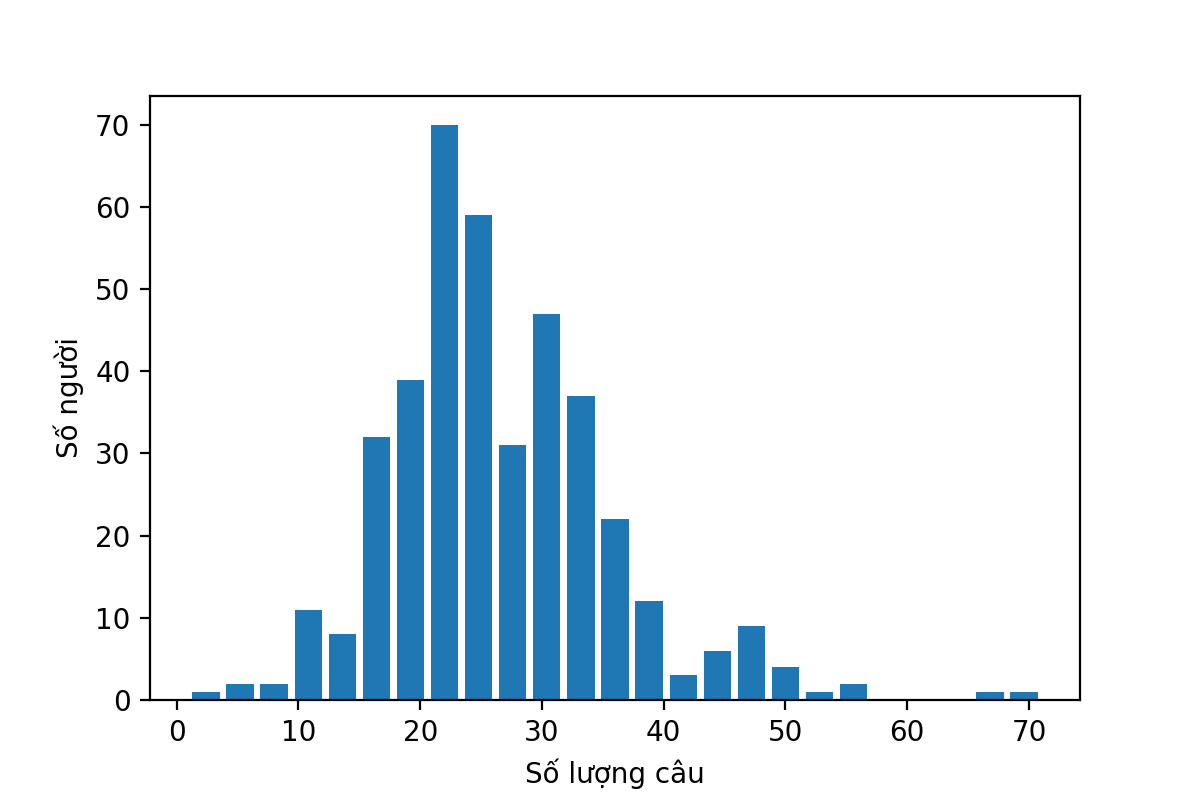
\includegraphics[width=0.8\textwidth]{images/zaloai.png}
  \caption{Biểu đồ phân phối số danh tính theo số câu nói của bộ dữ liệu ZaloAI}
  \label{fig:zaloai}
\end{figure}

VIVOS là tập giọng nói tiếng Việt phục vụ cho bài toán nhận dạng tiếng nói thu thập bởi phòng thí nghiệm khoa học máy tính AILAB từ trường Đại học Khoa học Tự nhiên - Đại học Quốc Gia TP.HCM \cite{VIVOS}. Tuy chủ đích của bộ dữ liệu là dành cho nhận dạng tiếng nói nhưng lại có nhãn danh tính cụ thể nên có thể sử dụng cho bài toán nhận dạng người nói. Tập huấn luyện VIVOS bao gồm 40 danh tính với trung bình \textit{253.5} câu nói mỗi người. Tập kiểm thử có 19 danh tính không trùng với tập huấn luyện với trung bình \textit{40} câu nói mỗi người. Chất lượng dữ liệu của VIVOS rất tốt do điều kiện thu âm được kiểm soát nên không yêu cầu xử lý gì thêm.

Bộ dữ liệu VLSP ASR 2020 \cite{VLSP} nằm trong chiến dịch đánh giá năm 2020 của Hiệp hội xử lý Ngôn ngữ và Tiếng nói tiếng Việt. Giống như VIVOS, VLSP ASR 2020 được thu thập và thiết kế cho bài toán nhận diện giọng nói nhưng có nhãn danh tính cho các câu nói. Tổng số danh tính trong VLSP ASR 2020 là $567$ người với trung bình $22.3$ câu mỗi người. Tuy nhiên, dữ liệu danh tính của bộ dữ liệu lại không được chuẩn xác và có nhiều vấn đề tương tự như bộ ZaloAI. Những vấn đề này được giải quyết bằng phương pháp mô tả trong \ref{noise-removal}.

\subsection{Cải thiện chất lượng bộ dữ liệu} \label{noise-removal}
Hai bộ ZaloAI và VLSP có tổng cộng gần 1 nghìn danh tính và hơn 20 nghìn câu. Do vậy, việc kiểm tra dữ liệu rất khó khăn và tốn thời gian. Việc này còn trở nên khó khăn hơn khi đánh giá bằng tai người, ví dụ để phân biệt giọng của 2 người cùng là nam, giọng trầm miền bắc thì cần sự tập trung cao độ để tìm điểm khác biệt. Vì thế, đồ án phân tích ma trận tương đồng của các câu nói để tìm ra sự không nhất quán từ đó thu hẹp phạm vi kiểm tra.

Cho một tập biểu diễn $n$ đoạn âm thanh đầu vào $\bm{V} = \{\bm{v}_0, \bm{v}_1, ..., \bm{v}_{n-1}\}$, sử dụng độ tương đồng cô-sin, ma trận tương đồng cho các đoạn tiếng nói được tính theo công thức \ref{eq:experiments1}. Ví dụ một ma trận tương đồng trong Hình \ref{fig:similarity-example}, đường chéo chính có giá trị tương đồng là 1 do so sánh mỗi câu với chính câu đó.

\begin{equation} \label{eq:experiments1}
  \bm{S}_{i,j} = cos(\bm{v}_i, \bm{v}_j) = \dfrac{\bm{v}_i \cdot \bm{v}_j}{\|\bm{v}_i\| \|\bm{v}_j\|}, 0 \leq i,j \le n
\end{equation}

\begin{figure}[h]
  \centering
  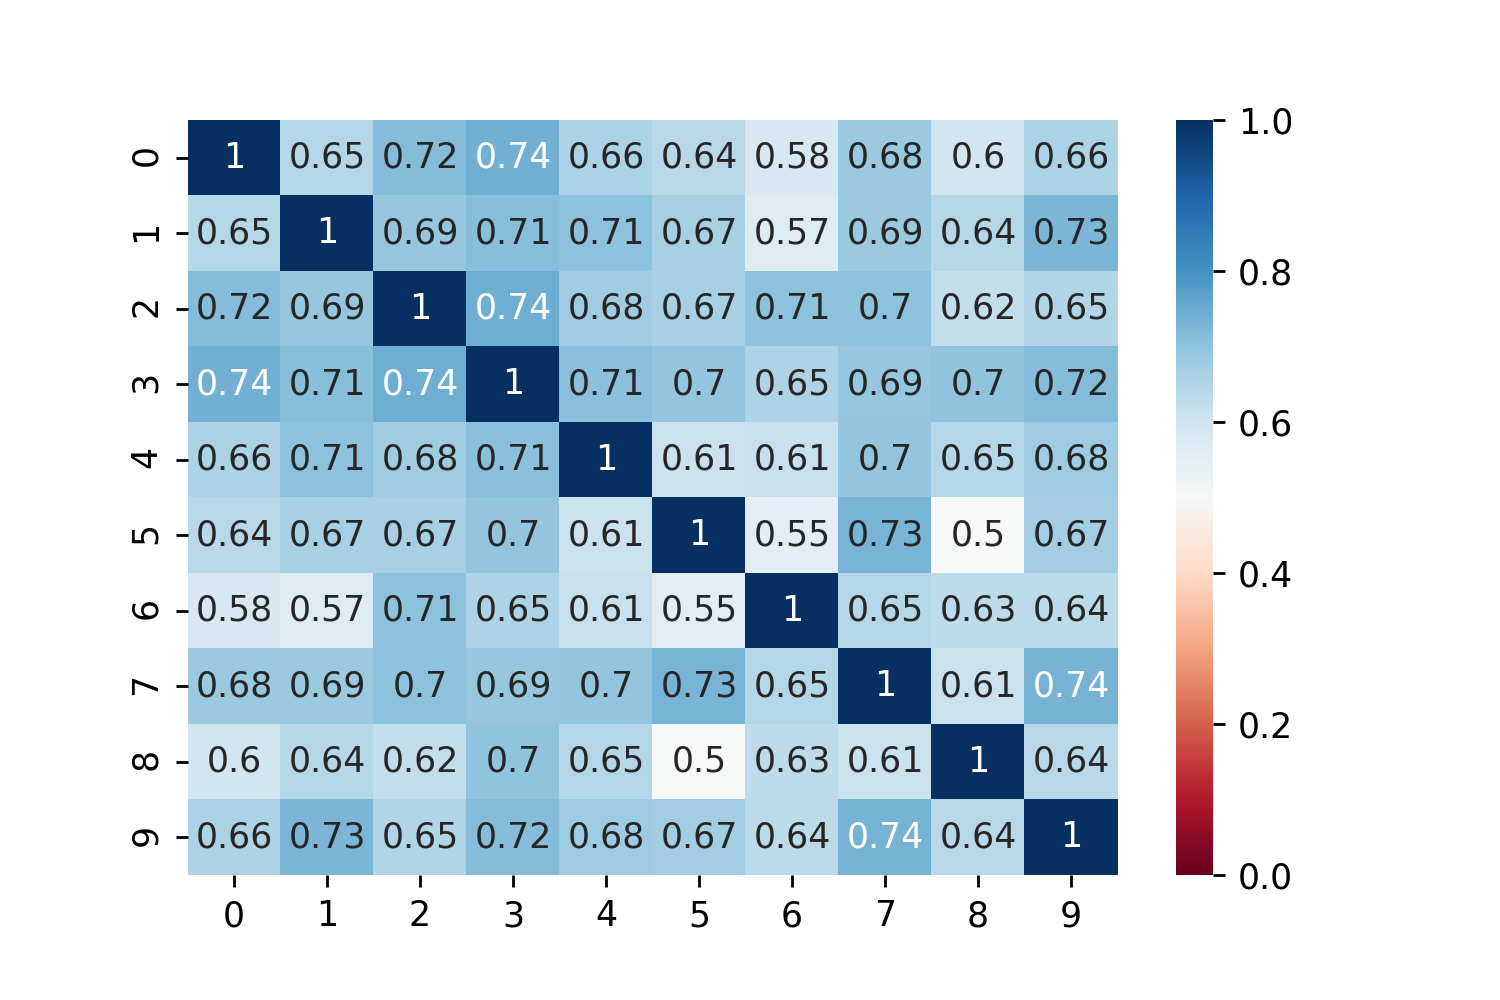
\includegraphics[width=0.8\textwidth]{images/similarity.png}
  \caption{Ma trận tương đồng cho một tập 10 đoạn âm thanh của một người}
  \label{fig:similarity-example}
\end{figure}

Ma trận tương đồng được áp dụng khá rộng rãi, trong đó, phổ biến nhất là phân tích âm nhạc dựa trên nội dung \cite{silva2018fast}, phân tích văn bản \cite{hussain2010improved} và tin sinh \cite{bustamam2018implementation}. Các kĩ thuật được sử dụng chủ yếu là phân cụm và phân đoạn. Trong đồ án, tác giả chỉ sử dụng phân tích đơn thuần để tìm ra các người nói, câu nói có khả năng bị gán nhãn sai.

\subsubsection{Loại bỏ người nói không hợp lệ}
Việc loại bỏ một danh tính có thể do nhiều lý do: nhiều câu nói không thuộc về người đó, chất lượng âm thanh kém, môi trường xung quanh ồn ào, tệp âm thanh bị hư hại qua đường truyền hoặc thiết bị, ... Các nguyên nhân này dẫn đến việc chất giọng của danh tính không được đảm bảo gây bất lợi cho việc huấn luyện mô hình. Một số danh tính có số lượng câu có vấn đề lớn, làm sạch và loại bỏ từng câu bằng việc nghe rất tốn thời gian và công sức. Do vậy, việc loại bỏ hẳn những danh tính này là cân thiết. Khi nhìn vào ma trận tương đồng của một danh tính, có thể thấy được và loại bỏ những danh tính không hợp lệ. Ma trận tương đồng của một người hợp lệ và bị loại bỏ có thể được thấy trong Hình \ref*{fig:similarity-example} và Hình \ref*{fig:similarity-utt-eer} tương ứng.

\begin{figure}[h]
  \centering
  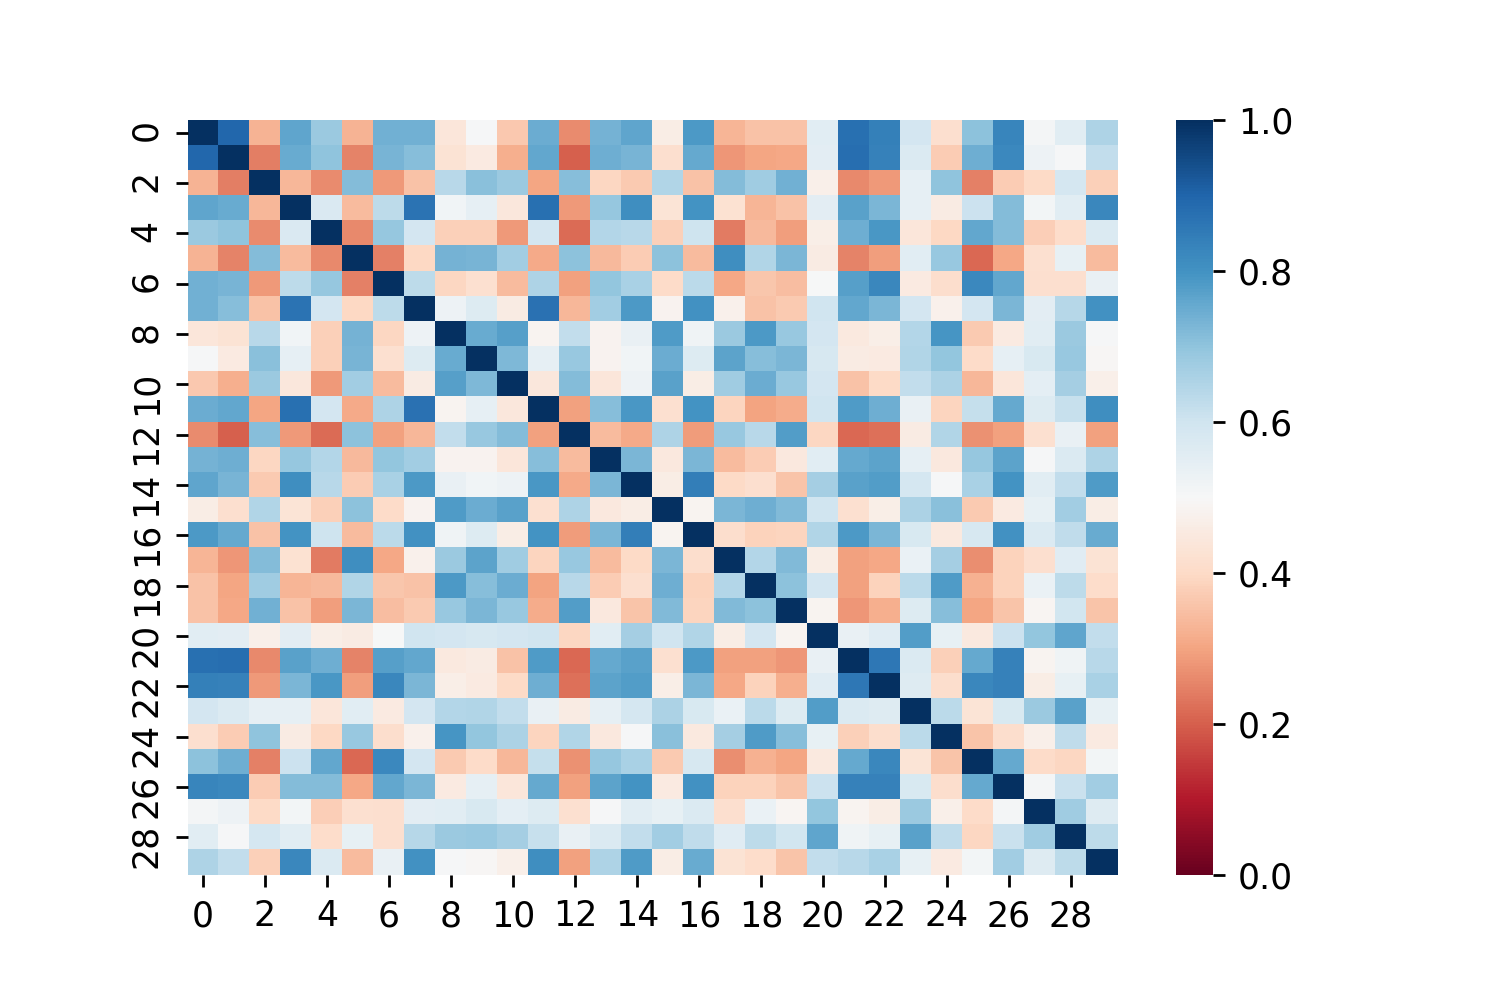
\includegraphics[width=0.8\textwidth]{images/similarity-spk-eer.png}
  \caption{Ma trận tương đồng của một danh tính bị loại bỏ}
  \label{fig:similarity-utt-eer}
\end{figure}

\subsubsection{Loại bỏ đoạn tiếng nói không hợp lệ}
Các đoạn tiếng nói không hợp lệ bao gồm sai nhãn danh tính, độ dài quá ngắn, tiếng ồn xung quanh quá lớn hay trong một đoạn có giọng của nhiều người khác nhau. Các đoạn này làm cho việc huấn luyện mô hình gặp khó khăn và giảm chất lượng của mô hình đầu ra. Lấy ma trận tương đồng của một người có câu nói không hợp lệ (Hình \ref{fig:similarity-utt-eer}) làm ví dụ, để lọc ra đoạn có chỉ số 6 khá đơn giản bằng cách lấy một ngưỡng thấp (ví dụ 0.3). Những câu có độ tương đồng so với những câu khác của một danh tính mà dưới ngưỡng này ta sẽ xem là không hợp lệ. Tuy nhiên, cách này không hợp lý với những câu như câu chỉ số 2 trong Hình \ref*{fig:similarity-utt-eer}, có điểm nằm trong khoảng 0.4 - 0.6. Tuy có điểm tương đồng khá cao nhưng những câu này cũng cần được kiểm tra. Những câu này có thể được tìm thấy bằng cách phát hiện ngoại lệ sử dụng khoảng trong tứ phân vị (Interquartile range) \cite{yang2019outlier}.

Với, Q1, Q3 lần lượt là tứ phân vị thứ nhất và thứ ba của tập điểm trung bình của các câu $a_i = \dfrac{1}{n} \sum_{j=0, j \neq i}^{n-1}\bm{S}_{i,j}$, dựa trên khoảng trong tứ phân vị, đoạn điểm tương đồng hợp lệ cho tập điểm $\bm{a}$ được tính như sau:

\begin{equation}
  a_{min} = Q1 - 1.5 * IQR;\ a_{max} = Q3 + 1.5 * IQR
\end{equation}

\begin{equation}  
  IQR = Q3 - Q1
\end{equation}

Các câu có điểm trung bình $a_i$ nằm ngoài đoạn $[a_{min}, a_{max}]$ được đánh dấu và cần nghe lại để quyết định có loại bỏ hay không. 

\begin{figure}[h]
  \centering
  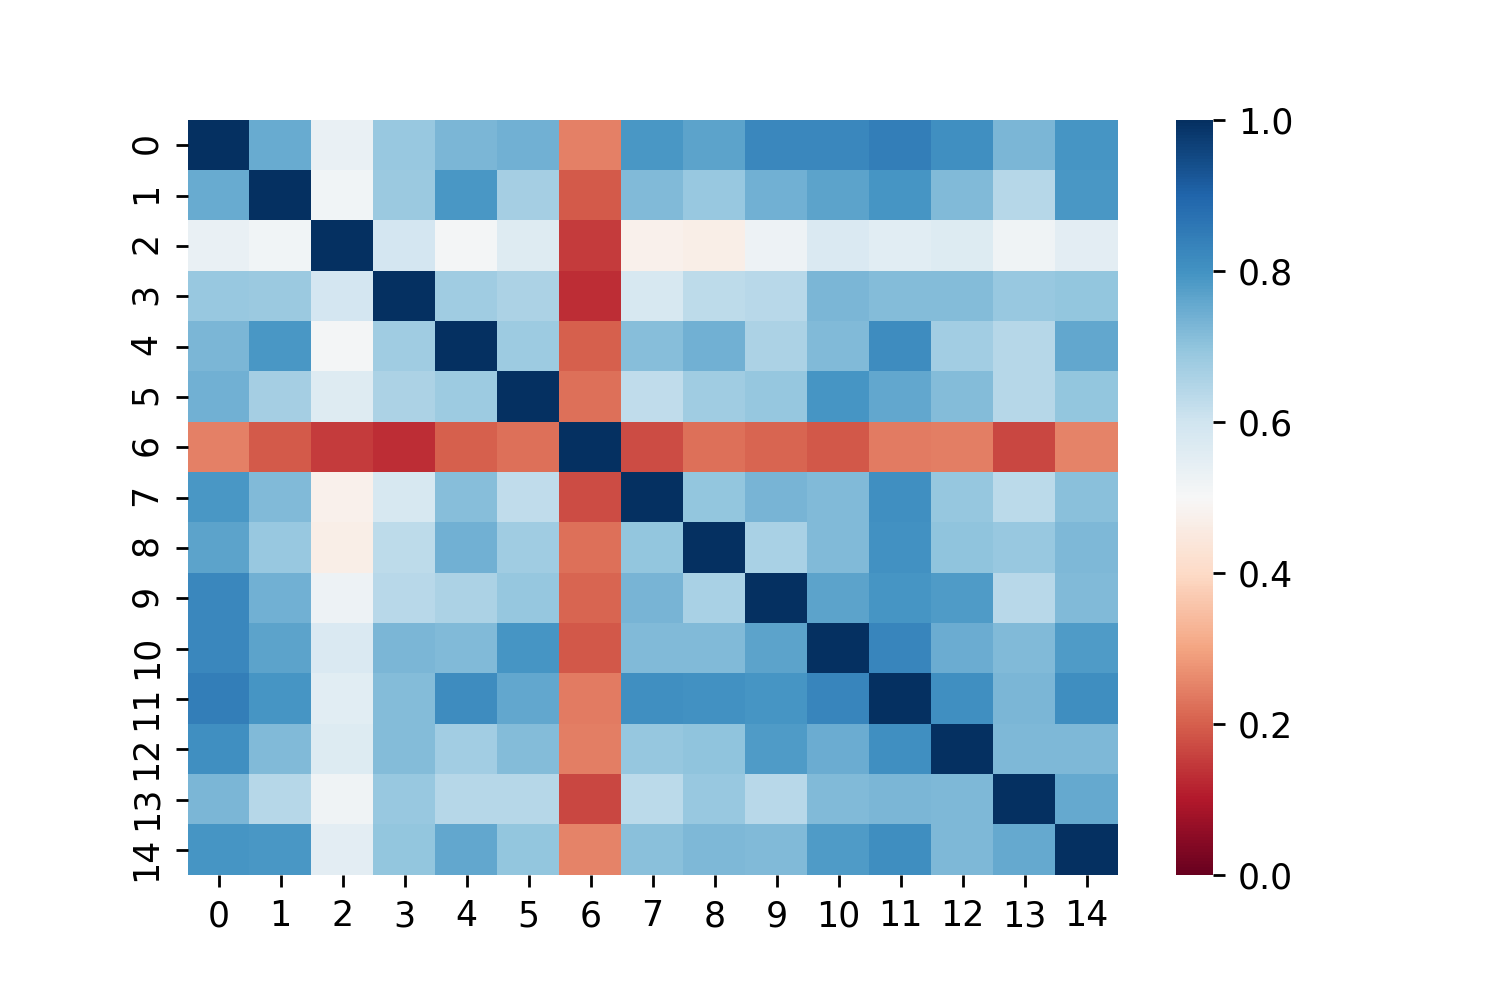
\includegraphics[width=0.8\textwidth]{images/similarity-utt-eer.png}
  \caption{Ma trận tương đồng của một danh tính có đoạn âm thanh không hợp lệ}
  \label{fig:similarity-utt-eer}
\end{figure}

\subsubsection{Hợp nhất người nói có cùng danh tính}
Do các bộ dữ liệu được thu thập một cách độc lập, có khả năng người nói trong bộ dữ liệu này trùng với bộ kia. Hơn nữa, một người đã tồn tại trong cơ sở dữ liệu cũng có khả năng được yêu cầu thu lại. Các cặp người nói trùng danh tính có thể được tìm dựa vào ma trận tương đồng chéo. Từ Hình \ref*{sub@fig:similarity-cross-sub1} mô tả ma trận tương đồng của người nói 52-M-31 và 64-M-30, có thể thấy rõ đây là 2 người khác nhau do ma trận tương đồng chéo (phần màu đỏ) có điểm tương đồng rất thấp. Ngược lại, trong Hình \ref*{fig:similarity-cross-sub2}, 2 người có nhãn khác nhau là 64-M-30 và 636-M-30 thực chất là cùng một người với ma trận tương đồng chéo nằm trong ô màu đỏ. Có nhiều cặp câu điểm tương đồng cao (ô xanh đậm) nhưng không đạt tới $1.0$ như trên đường chéo chính do cơ bản có cùng nội dung nhưng khác biệt đến từ sự biến đổi nhất định trong quá trình xử lý. Các cặp người nói có giá trị trung bình của ma trận tương đồng chéo lớn hơn $0.7$ yêu cầu được nghe lại và ra quyết định để hợp nhất.

\begin{figure}
  \centering
  \begin{subfigure}{.5\textwidth}
    \centering
    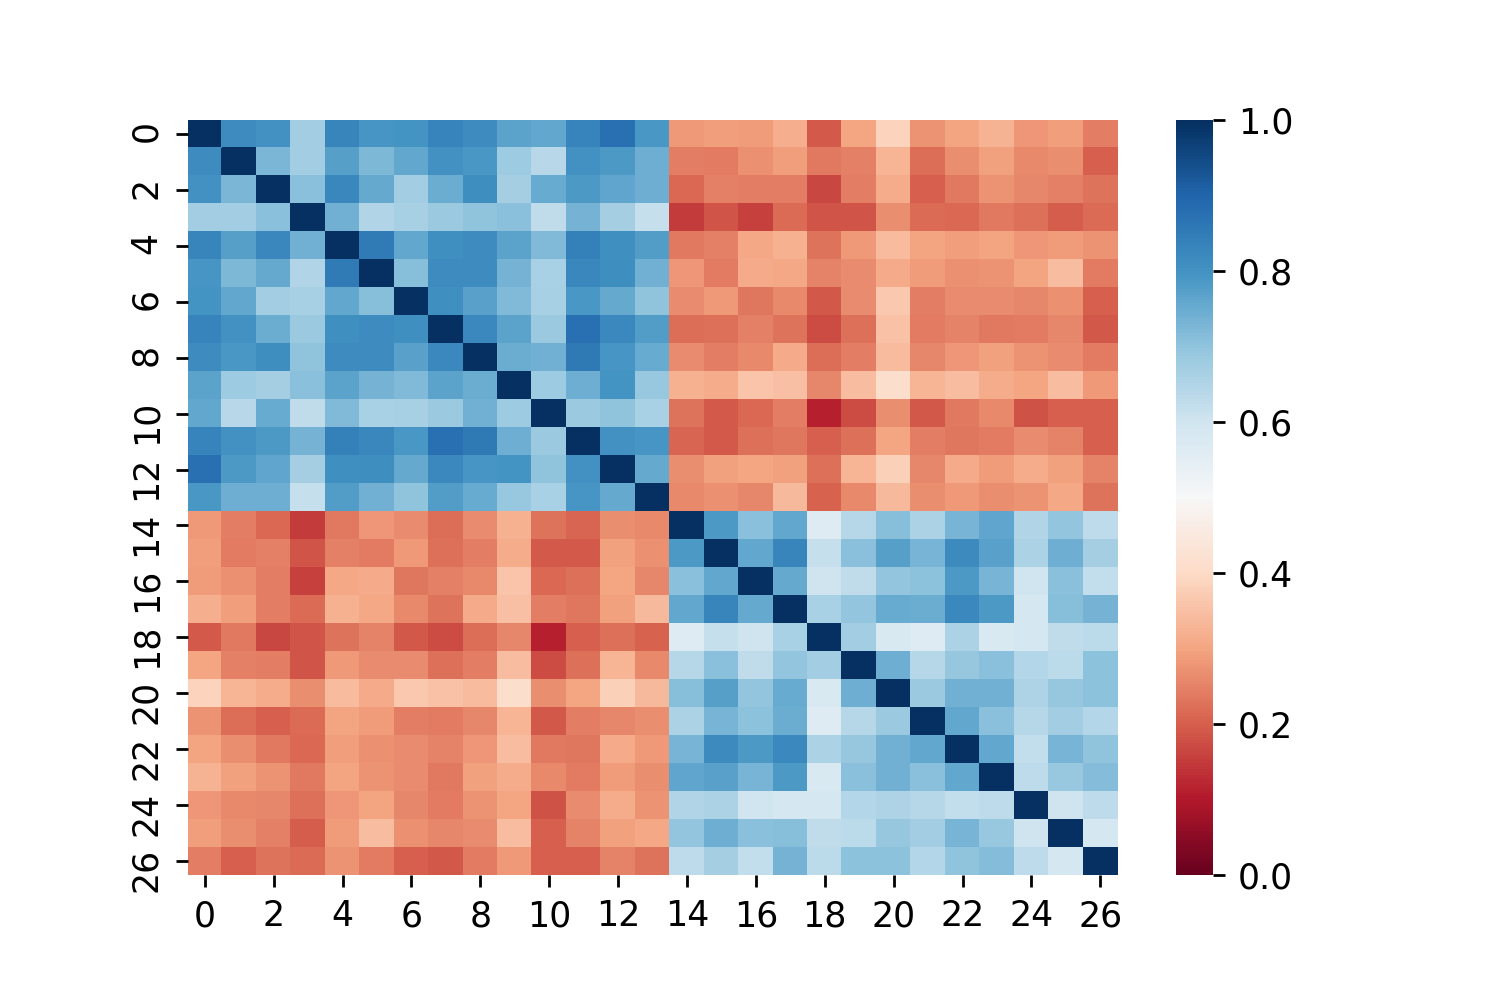
\includegraphics[width=\textwidth]{images/similarity-cross1.png}
    \caption{Ma trận tương đồng của 52-M-31 và 64-M-30}
    \label{fig:similarity-cross-sub1}
  \end{subfigure}%
  \begin{subfigure}{.5\textwidth}
    \centering
    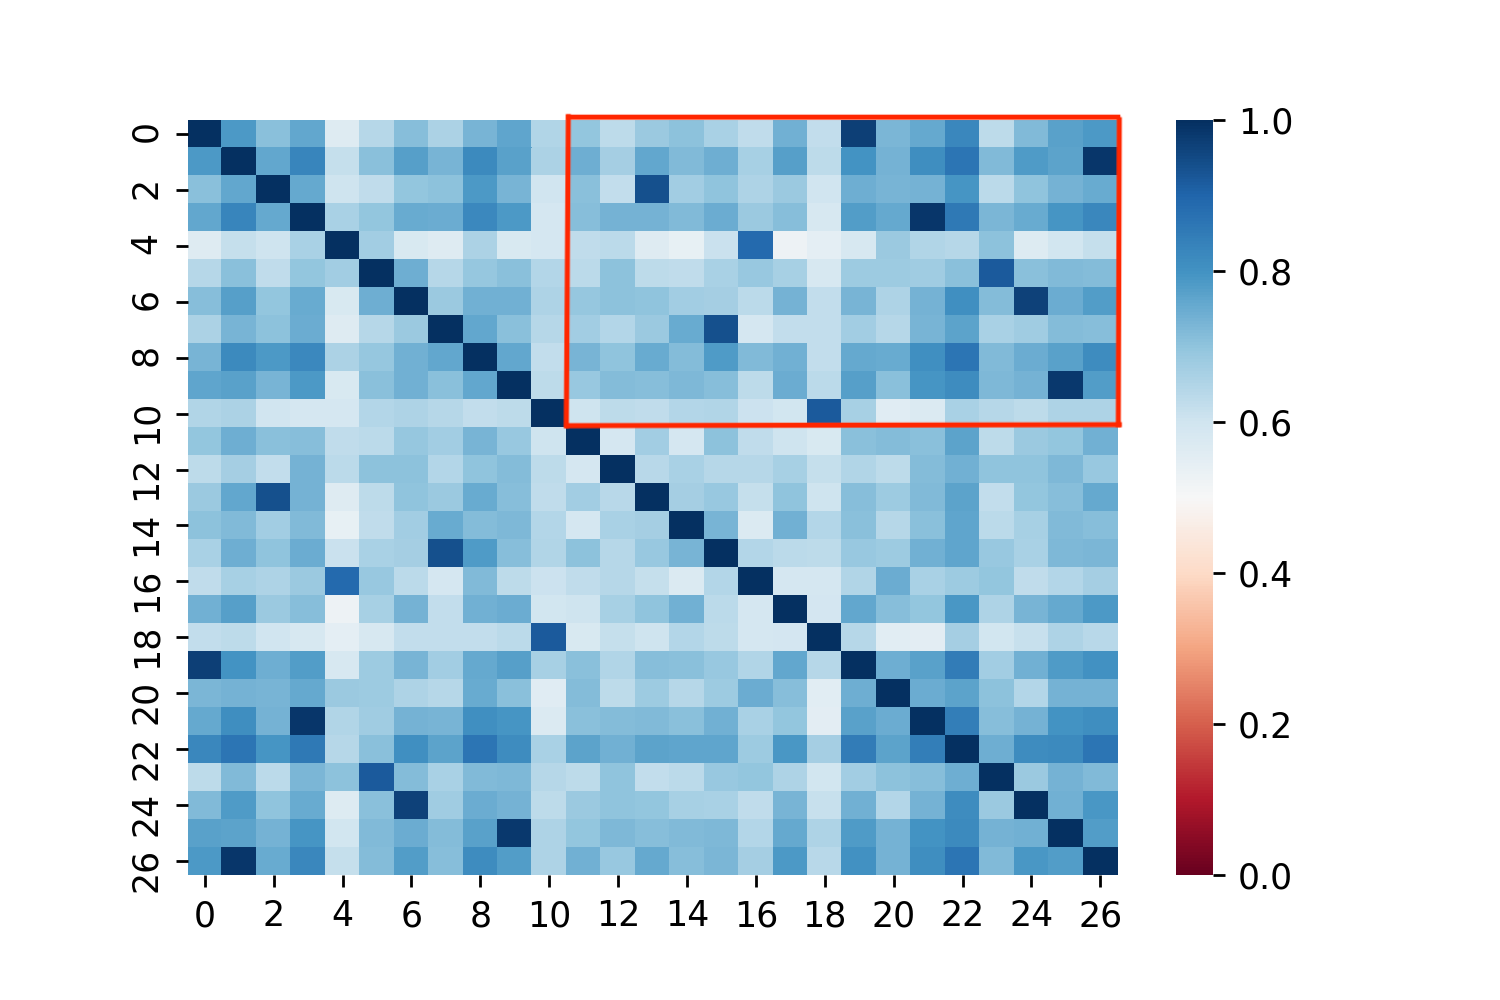
\includegraphics[width=\textwidth]{images/similarity-cross2.png}
    \caption{Ma trận tương đồng của 64-M-30 và 636-M-30}
    \label{fig:similarity-cross-sub2}
  \end{subfigure}
  \caption{}
  \label{fig:similarity-cross-sub2}
\end{figure}

% \subsubsection{Tổng kết cải thiện chất lượng dữ liệu}

Bảng \ref*{tab:data-filtering} tổng kết thông tin sàng lọc dữ liệu. Số người nói bị loại bỏ chiếm \TODO{stat} tổng số người nói, số người nói được hợp nhất chiếm \TODO{stat} tổng số người nói, số câu nói bị loại bỏ chiếm \TODO{stat} tổng số câu. 

\begin{table}[h]
  \centering
  \begin{tabular}{|l|r|r|r|}
    \hline
    \textbf{Bộ dữ liệu}& \textbf{Số danh tính loại bỏ} & \textbf{Số danh tính hợp nhất} & \textbf{Số câu loại bỏ} \\
    \hline
    ZaloAI  & 0   & 51  & 1,066 \\
    VIVOS   & 0   & 0   & 2 \\
    VLSP    & 65  & 33  & 549 \\
    Tổng    & 65  & 84  & 1,617 \\
    \hline
  \end{tabular}
  \caption{placeholder}
  \label{tab:data-filtering}
\end{table}



\subsection{Bộ dữ liệu thực nghiệm}
Sau khi loại bỏ các danh tính không phù hợp, hợp nhất người nói có cùng danh tính và loại bỏ các câu vấn đề, bộ dữ liệu thực nghiệm đã có chất lượng tương đối tốt. Tổng số lượng người nói là 1110, chia thành 3 tập: tập huấn luyện (training set) gồm 1031 người nói, tập kiểm thử (validation set) gồm 20 người, tập kiểm tra (test set) gồm 59 người nói. Người nói trong tập kiểm thử và 40 người trong tập kiểm tra được lấy ngẫu nhiên trong bộ ZaloAI với điều kiện cân bằng giới tính nam - nữ. 19 người còn lại trong tập kiểm tra là tập kiểm thử của bộ dữ liệu VIVOS.

\section{Chi tiết cài đặt thực nghiệm}
\subsubsection{Thông số huấn luyện mô hình}
Các thực nghiệm trong mục tiếp theo đều được chạy trên cùng bộ thông số như sau:
\begin{itemize}
  \item Mạng trích xuất đặc trưng: ResNet
  \item Lớp tổng hợp: Tổng hợp thống kê tập trung
  \item Batch size: 100
\end{itemize}

\subsubsection{Môi trường lập trình}
Để cài đặt thực nghiệm, tác giả sử dụng ngôn ngữ lập trình Python kết hợp với thư viện PyTorch phiên bản 1.7.1. PyTorch là thư mã nguồn mở của Facebook được xây dựng trên ngôn ngữ lập trình Lua. PyTorch cho phép người dùng xây dựng, tuỳ biến mô hình ở cả cấp cao và cấp thấp với thiết kế trực quan.

\subsubsection{Môi trường thực nghiệm}
Để thực hiện huấn luyện các mô hình, tác giả sử dụng Google Colaboratory: Hệ điều hành Ubuntu 18.04, 2vCPU Intel Xeon 2.2 Ghz, RAM 25GB, GPU Tesla T4 15GB.

\section{Kết quả thực nghiệm và đánh giá}
Trong phần này tác giả sử dụng tỉ lệ lỗi bằng nhau (Equal error rate - EER) để đánh giá hiệu năng của các mô hình thực nghiệm. EER là điểm nằm trên đường ROC mà có tỉ lệ dương tính giả (ví dụ bình thường được coi là bất thường) và tỉ lệ âm tính giả (ví dụ bất thường được xem là bình thường). Hệ thống nhận dạng càng tốt thì có EER càng nhỏ.

Tác giả thực hiện nhiều trường hợp thực nghiệm khác nhau với mục tiêu huấn luyện mô hình nhận dạng người nói một cách có hiệu quả trên tiếng Việt. . Thực nghiệm 5 kiểm tra tính hiệu quả của hàm mất mát AP với margin khác nhau. Mặc định, các thông số \TODO{...}:
\begin{itemize}
  \item Các mô hình được finetune từ mô hình train sẵn trong \cite{}.
\end{itemize}

\subsubsection{Thực nghiệm 1: làm sạch dữ liệu}
Bảng \ref*{tab:experiment-clean} mô tả kết quả thực nghiệm với dữ liệu ban đầu và dữ liệu đã được sàng học như đã trình bày trong \ref*{noise-removal}. Như có thể thấy, kết quả huấn luyện trên tập đã sàng lọc cải thiện 0.93\% EER so với dữ liệu gốc. Do vậy, các thực nghiệm về sau sẽ sử dụng bộ dữ liệu đã qua sàng lọc.

\begin{table}[h]
  \centering
  \begin{tabular}{|l|r|}
    \hline
    \textbf{Dữ liệu}& \textbf{EER trên tập kiểm tra}\\
    \hline
    Gốc & 6.790\% \\
    Cải thiện chất lượng & 5.860\% \\
    \hline
  \end{tabular}
  \caption{placeholder}
  \label{tab:experiment-clean}
\end{table}

\subsubsection{Thực nghiệm 2: Phương thức huấn luyện}
Trong thực nghiệm này, tác giả tiến hành khảo sát các phương thức huấn luyện mô hình. Bảng \cite{tab:experiment-training} mô tả kết quả với các trường hợp khác nhau. Do số người nói trong bộ dữ liệu tiếng Việt ít hơn hẳn so với người nói tiếng Anh trong bộ dữ liệu VoxCeleb, huấn luyện không tập trung đủ để tìm ra các điểm hữu dụng phân biệt người nói tiếng Việt, dẫn đến mô hình huấn luyện từ đầu kết hợp hai bộ dữ liệu đạt kết quả tệ hơn. Có thể thấy finetune bằng riêng dữ liệu tiếng Việt cho kết quả vượt trội so với huấn luyện từ đầu bằng bộ dữ liệu tiếng Việt hoặc kết hợp VoxCeleb (dữ liệu tiếng Anh) với EER 4.775\%. Các thử nghiệm phía sau sử dụng phương pháp finetune.

\begin{table}[h]
  \centering
  \begin{tabular}{|l|r|}
    \hline
    \textbf{Phương pháp}& \textbf{EER trên tập kiểm tra}\\
    \hline
    Pretrain & 10.60\% \\
    Scratch + vn data + VoxCeleb & 6.294\% \\
    Scratch + vn data & 5.860\% \\
    Finetune & \textbf{4.775\%} \\
    \hline
  \end{tabular}
  \caption{placeholder}
  \label{tab:experiment-training}
\end{table}

\subsubsection{Thực nghiệm 3: Khử nhiễu đầu vào}

\begin{table}[h]
  \centering
  \begin{tabular}{|l|r|}
    \hline
    \textbf{Dữ liệu}& \textbf{EER trên tập kiểm tra}\\
    \hline
    Nhiễu âm thanh & 4.775\% \\
    Khử nhiễu âm thanh & \textbf{4.215\%} \\
    \hline
  \end{tabular}
  \caption{placeholder}
  \label{tab:experiment-denoising}
\end{table}

\subsubsection{Thực nghiệm 4: Hàm tối ưu}

\begin{table}[h]
  \centering
  \begin{tabular}{|l|r|}
    \hline
    \textbf{Dữ liệu}& \textbf{EER trên tập kiểm tra}\\
    \hline
    ADAM & 4.215\% \\
    SGD & \textbf{2.930\%} \\
    \hline
  \end{tabular}
  \caption{placeholder}
  \label{tab:experiment-optimizer}
\end{table}

\subsubsection{Thực nghiệm 5: Hàm mất mát}

\begin{table}[h]
  \centering
  \begin{tabular}{|l|r|}
    \hline
    \textbf{hmm}& \textbf{EER trên tập kiểm tra}\\
    \hline
    AP & 2.930\% \\
    AP (m=0.1) & 2.789\% \\ 
    AP (m=0.2) & \textbf{2.749\%} \\
    AP (m=0.3) & 2.754\% \\
    AP (m=0.4) & 2.804\%\\
    AP (m=0.5) & 2.892\%\\
    \hline
  \end{tabular}
  \caption{placeholder}
  \label{tab:experiment-loss}
\end{table}

- Visualizing embedding space with t-SNE (some speakers)
- DET curve